\documentclass{article}
\usepackage[margin=0.9in]{geometry}
\usepackage{graphicx}
\usepackage{booktabs}
\usepackage{amsmath}
\usepackage{hyperref}
\usepackage{xcolor}
\usepackage{listings}
\usepackage{caption}
\usepackage{parskip}
\usepackage{enumitem}
\usepackage{longtable}
\usepackage{tabularx}
\usepackage{float}
\usepackage{placeins}
\setlist{nosep, leftmargin=1.5em}
\hypersetup{colorlinks=true, linkcolor=blue, urlcolor=blue, citecolor=blue}
\lstset{basicstyle=\ttfamily\footnotesize, breaklines=true, columns=fullflexible, frame=single, framerule=0.2pt}
\captionsetup{font=small, labelfont=bf}
\renewcommand{\topfraction}{0.9}
\renewcommand{\bottomfraction}{0.8}
\renewcommand{\textfraction}{0.07}
\renewcommand{\floatpagefraction}{0.85}
\setcounter{topnumber}{3}
\setcounter{totalnumber}{5}
\newcommand{\runcvmedian}{0.2}
\newcommand{\runcvmean}{0.8}
\newcommand{\runcvmax}{9.7}
\newcommand{\runcvmaxpoint}{exp8 inlined n=4096 GFLOP/s}


\title{Project 1: SIMD Advantage Profiling\\[3pt]\large ECSE 4320/6320 Advanced Computer Systems}
\author{Demetrios Sotirelis}
\date{\today}

\emergencystretch=3em
\begin{document}
\maketitle

\begin{abstract}
  This report measures how much single instruction, multiple data (SIMD) auto-vectorization speeds up four single-precision kernels, $a\cdot x$ plus $y$ (SAXPY), dot product, elementwise multiply and a three-point stencil, on one core of an AMD Ryzen~9 9950X (Zen~5) at a measured 5.61\,GHz. The same source is built as scalar code and for 128-bit Streaming SIMD Extensions 2 (SSE2), 256-bit Advanced Vector Extensions 2 (AVX2) and 512-bit Advanced Vector Extensions 512 (AVX-512), with working sets from L1 to dynamic random-access memory (DRAM). In cache, AVX-512 makes SAXPY and multiply about ten times faster; in DRAM the gain is at most 1.3$\times$, because the scalar loops already use most of the bandwidth. A floating-point dot product the compiler reports as vectorized runs at scalar speed, a loop that calls an opaque function stays scalar, and large strides and gathers gain nothing or lose. A summary of results, a map from the grading rubric to this report and a requirements checklist are in the appendices.
\end{abstract}

\section{Reproducibility}\label{sec:repro}
The repository holds the sources (\texttt{src/}), the build, run and processing scripts (\texttt{scripts/}), the raw measurements (\texttt{data/raw}, \texttt{data/repeats}), the derived tables (\texttt{data/processed}) and the figures with the recorded environment and build flags (\texttt{results/}). These commands rebuild everything:
\begin{lstlisting}
powershell -File scripts\build.ps1                  # all ISA variants -> bin\  (flags: results\build_flags.txt)
powershell -File scripts\run_all.ps1                # all experiments, pinned -> data\raw\*.csv  (+ environment, clock log)
powershell -File scripts\run_all.ps1 -RawDir data\repeats\run2    # repeat runs (also run3)
powershell -File scripts\verify_vectorization.ps1   # compiler reports + disassembly -> results\vectorization_evidence\
python scripts\process_and_plot.py                  # raw -> processed tables, figures, report\generated\*.tex
python scripts\repeat_check.py                      # run-to-run variation
powershell -File scripts\run_counters.ps1          # elevated shell: hardware counters -> data\raw\counters\exp9_counters.csv
python scripts\process_counters.py                 # counters -> results\figE_counters.png, report\generated\table_counters_*.tex
\end{lstlisting}
The full suite runs as a set of separate processes, and \nolinkurl{scripts/repeat_check.py} compares the medians of 38 headline points. The median coefficient of variation is \textbf{\runcvmedian\%}. The two points that vary by about 9\% depend on where the allocator places the output array relative to the input, which could be attributed to 4\,KiB aliasing. Every conclusion is reproducible over every run.

\section{Methodology}\label{sec:method}
\subsection{Platform and measurement}\label{sec:platform}
{\small
\begin{longtable}{p{2.6cm}p{13.4cm}}
\toprule
Processor & AMD Ryzen 9 9950X: 16 cores on two core complex dies (CCDs), simultaneous multithreading (SMT) enabled. Per core two 512-bit fused multiply-add (FMA) units, a 48\,KiB L1 data cache (L1D), a 32\,KiB L1 instruction cache and a 1\,MiB L2; 32\,MiB of L3 per CCD \cite{amdhc,chips9950x} \\
Memory & 2 $\times$ 16\,GB double data rate 5 (DDR5) at 6000\,MT/s \\
Software & Windows 11 Home build 26200; g++ 16.2.0 from MSYS2 MinGW-w64, \texttt{-std=c++17 -static}; Python 3.12 \\
Frequency & Median 5.61\,GHz, with slight deviation as discussed later in the report. 5.61 GHz was used for every cycles-per-element value. \\
Pinning & One thread on logical processor 4, its SMT sibling idle, at high priority; 2.2\% background load. \\
Timing & \texttt{std::chrono::steady\_clock}; batches doubled to at least 2--10\,ms; 9--21 batches per point; plots show the median and interquartile range; three independent full runs. \\
Data & \texttt{mt19937\_64}, fixed seeds, uniform in $(-1,1)$; arrays 64-byte aligned unless alignment is the variable. \\
Units & Bandwidth counts the compulsory bytes per element: 12\,B for SAXPY and multiply, 8\,B for dot and the stencil. Throughput is in billions of floating-point operations (FLOP) per second (GFLOP/s). The roofline's true DRAM traffic also counts the write-allocate read of a separate output array. \\
\bottomrule
\end{longtable}
}

\subsection{Build variants and vectorization verification}\label{sec:verify}
Every variant compiles the same source; only these flags differ:
\begin{center}\small
\begin{tabular}{lp{6.0cm}p{6.6cm}}
\toprule
variant & flags & purpose \\
\midrule
scalar & \texttt{-O3 -march=native -fno-tree-vectorize -fno-tree-slp-vectorize} & scalar baseline that still uses FMA, so the gap measures SIMD only \\
SSE2 & \texttt{-O3 -march=x86-64} & gcc's default 128-bit target \\
AVX2 & \texttt{-O3 -mavx2 -mfma} & 256-bit \\
AVX-512 & \texttt{-O3 -march=native} & widest target for this processor \\
+ fast-math & \texttt{-O3 -march=native -ffast-math} & allows floating-point reordering \cite{gccdoc} \\
gather forced & \texttt{-O3 -march=native -mtune-ctrl=use\_gather} & allows the gather instruction gcc avoids on Zen~5 \\
\bottomrule
\end{tabular}
\end{center}
gcc's \texttt{-fopt-info-vec} reports give the vector width each build uses for each loop; the full version is in \nolinkurl{results/vectorization_evidence/summary_table.md}.
\begin{center}\footnotesize
\begin{tabular}{lcccc}
\toprule
loop (f32) & SSE2 & AVX2 & AVX-512 & AVX-512 + fast-math \\
\midrule
saxpy, mul, stencil & 16 B & 32 B & 64 B, masked epilogue & 64 B, masked epilogue \\
dot (f32) & 16 B & 32 B & 64 B (but see below) & 64 B, 4 vector accumulators \\
dot (i32) & -- & -- & 64 B & -- \\
strided $x[iS]$, $S=2,4,8$ & 16 B ($S\le4$ only) & 32 B & 64 B (shuffles, not gathers) & 64 B \\
strided $x[iS]$, $S=16$ & \multicolumn{4}{c}{\textbf{not vectorized}} \\
\texttt{x[idx[i]]} gather & \multicolumn{3}{c}{\textbf{not vectorized} (``no vectype for stmt'')} & vectorized only with \texttt{use\_gather} \\
\bottomrule
\end{tabular}
\end{center}
\begin{lstlisting}
saxpy<float>, AVX-512:  vbroadcastss zmm2,xmm2 ; vmovups zmm0,[rdx+rax] ; vfmadd213ps zmm0,zmm2,[rcx+rax] ; vmovups [rcx+rax],zmm0
   masked epilogue:     vmovups zmm0{k1}{z},[...] ; vfmadd132ps zmm0{k1}{z},zmm1,zmm2 ; vmovups [...]{k1},zmm0
dot<float>, default FP: vmulps zmm1,zmm1,[rcx+rax]  (16 products at once)
                        vaddss xmm0,xmm0,xmm1 ; vshufps/vunpckhps/vextractf32x4 ...; vaddss xmm0,xmm0,xmm4 ; ...  (16 SEQUENTIAL scalar adds)
dot<float>, -ffast-math: vfmadd231ps zmm1,zmm4,[rcx] ; vfmadd231ps zmm2,zmm5,[rcx+0x40] ...  (independent accumulators)
\end{lstlisting}
gcc's ``64 byte vectors'' are 512-bit ZMM registers holding 16 f32 values. SAXPY copies $a$ into every lane once, then per 16 elements loads $x$, computes $a\cdot x+y$ in one FMA that reads $y$ from memory, and stores; the leftover elements get one masked pass, so there is no scalar cleanup loop. The default dot product forms 16 products at once but adds them one at a time with \texttt{vaddss}, because C++ requires floating-point additions in source order; \texttt{-ffast-math} lifts that rule and gcc keeps independent vector accumulators. Strides 2--8 use contiguous loads and \texttt{vpermt2ps} shuffles, not gathers. The hardware counters of Sec.~\ref{sec:counters} confirm that the vector code ran.

\subsection{Hardware counters}\label{sec:countermethod}
Windows has no \texttt{perf}, but Event Tracing for Windows (ETW) logs the performance counters at every context switch; Windows Performance Recorder (WPR) records the trace and \texttt{tools/etl\_pmc.cpp} decodes it, so nothing is installed and no setting changes. Each configuration runs twice with different call counts, and the difference removes setup costs; there is one differenced run per configuration, without error bars. The counters are retired instructions, cycles, loads and L1D fills by source \cite{perfzen5}, first checked on a pointer chase with a known miss pattern. Windows' built-in miss counters read zero, and there are no vector-instruction or memory-controller counters.

\subsection{Correctness validation}\label{sec:valid}
Before timing, every binary checks all four kernels in f32, f64 and i32 against plain reference loops with long-double accumulation, at 21 sizes, mostly not multiples of a vector width, and three offsets, two of them misaligned. The tolerance is the standard summation error bound, which holds for any addition order and so covers the fast-math dot product. Canary values around each output array catch out-of-bounds stores from masked tails; any failure aborts the run. The strided and gather kernels are checked bit for bit, the FMA peak loop against a double-precision recurrence, and the function-call loop of Sec.~\ref{sec:neg} against its inlined twin. Each build reaches nearly its theoretical FLOP per cycle (Tab.~\ref{tab:ceil}), and a dependent-add chain runs at the 2-cycle add latency reported for Zen~5 \cite{amdhc}.

\section{Hypotheses}\label{sec:hyp}
The predictions draw on the published specifications in Sec.~\ref{sec:platform}; the outcome column points to the evidence.
\begin{center}\small
\begin{tabularx}{\linewidth}{@{}lXX@{}}
\toprule
& \textbf{Prediction} & \textbf{Outcome} \\
\midrule
1 & \textbf{Scalar vs.\ SIMD:} scalar code sustains about one element per cycle; L1 load and store bandwidth caps unit-stride kernels at 8--12$\times$, not the ideal 16$\times$. & Mostly held. Wider vectors gave nothing once the data sat in L2, and the \texttt{-ffast-math} dot far exceeded the predicted gain (Sec.~\ref{sec:locality}). \\
2 & \textbf{Alignment and tail:} split cache lines cost 15--30\% with 64-byte vectors; the tail matters only for short loops. & Held; the AVX-512 misalignment penalty slightly exceeded the range (Sec.~\ref{sec:align}). \\
3 & \textbf{Stride and gather:} the gain shrinks with stride, as each line holds fewer useful elements, and vanishes for gathers. & Held but understated: at large strides and with forced gathers SIMD was slower than scalar (Sec.~\ref{sec:stride}). \\
4 & \textbf{Data type:} f64 reaches half the element rate of f32, having half the lanes; i32 matches f32. & Held (Sec.~\ref{sec:dtype}). \\
5 & \textbf{Roofline:} streaming kernels are memory-bound at DRAM sizes, and the dot product behaves like SAXPY. & Held for the streaming kernels; \textbf{wrong} for the dot product, which is limited by add latency (Sec.~\ref{sec:roofline}, \ref{sec:neg}). \\
6 & \textbf{Counters:} instructions per element fall with the lane count; line fills match the traffic model for scalar and SIMD; a vectorized floating-point reduction retires fewer instructions without fewer cycles. & Held; SSE2 cut the instruction count by less than its lane count (Sec.~\ref{sec:counters}). \\
\bottomrule
\end{tabularx}
\end{center}

\section{Results}\label{sec:results}
\subsection{Scalar vs.\ SIMD across working-set sizes}\label{sec:locality}
\begin{figure}[!htb]\centering
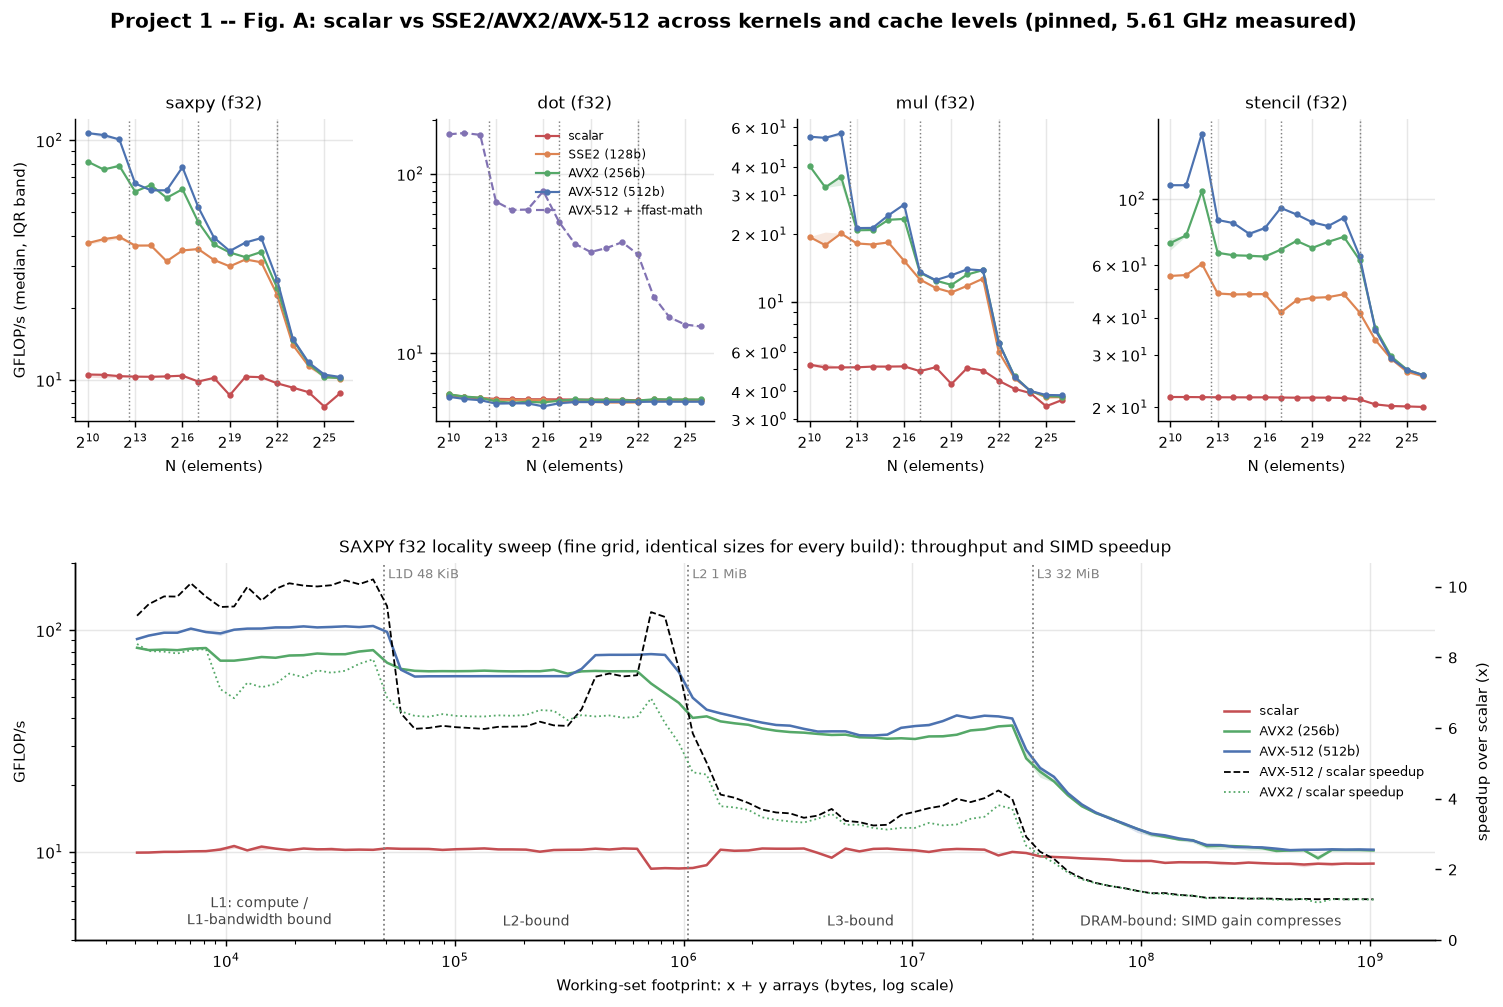
\includegraphics[width=\linewidth]{../results/figA_scalar_vs_vector_and_locality.png}
\caption{Top: throughput of the four kernels (f32) for each build (+\texttt{-ffast-math} for dot), $N=2^{10}$--$2^{26}$; dotted lines mark the L1D, L2 and L3 capacities for two f32 arrays. Bottom: fine SAXPY sweep with identical sizes for every build, and the resulting speedup.}\label{fig:A}
\end{figure}
\begin{table}[!htb]\centering\small
\begin{tabular}{llrrrrrrr}
\toprule
kernel & level & scalar & SSE2 & AVX2 & AVX-512 & +fast-math & cyc/elem & cyc/elem \\
 & ($N$) & GFLOP/s & $\times$ & $\times$ & $\times$ & $\times$ & scalar & AVX-512 \\
\midrule
saxpy & L1 ($2^{12}$) & 10.37 & 3.81 & 7.54 & 9.72 & 11.96 & 1.08 & 0.11 \\
 & L2 ($2^{16}$) & 10.42 & 3.33 & 6.00 & 7.42 & 7.38 & 1.08 & 0.15 \\
 & L3 (eff.) ($2^{20}$) & 10.32 & 3.08 & 3.15 & 3.63 & 3.20 & 1.09 & 0.30 \\
 & DRAM ($2^{26}$) & 8.81 & 1.15 & 1.16 & 1.17 & 1.15 & 1.27 & 1.09 \\
\addlinespace
dot & L1 ($2^{12}$) & 5.60 & 1.00 & 1.01 & 0.98 & 29.44 & 2.00 & 2.05 \\
 & L2 ($2^{16}$) & 5.53 & 0.99 & 0.96 & 0.91 & 14.48 & 2.03 & 2.22 \\
 & L3 (eff.) ($2^{20}$) & 5.50 & 0.97 & 1.00 & 0.97 & 7.02 & 2.04 & 2.10 \\
 & DRAM ($2^{26}$) & 5.46 & 1.01 & 1.01 & 0.98 & 2.58 & 2.06 & 2.10 \\
\addlinespace
mul & L1 ($2^{12}$) & 5.11 & 3.95 & 7.08 & 11.03 & 9.76 & 1.10 & 0.10 \\
 & L2 ($2^{16}$) & 5.16 & 2.95 & 4.54 & 5.26 & 5.27 & 1.09 & 0.21 \\
 & L3 (eff.) ($2^{20}$) & 5.08 & 2.32 & 2.61 & 2.75 & 2.74 & 1.11 & 0.40 \\
 & DRAM ($2^{26}$) & 3.65 & 1.03 & 1.04 & 1.05 & 1.04 & 1.54 & 1.46 \\
\addlinespace
stencil & L1 ($2^{12}$) & 21.62 & 2.80 & 4.91 & 7.67 & 7.85 & 1.30 & 0.17 \\
 & L2 ($2^{16}$) & 21.60 & 2.22 & 2.97 & 3.70 & 3.73 & 1.30 & 0.35 \\
 & L3 (eff.) ($2^{20}$) & 21.54 & 2.17 & 3.33 & 3.77 & 3.99 & 1.30 & 0.35 \\
 & DRAM ($2^{26}$) & 20.05 & 1.27 & 1.28 & 1.28 & 1.28 & 1.40 & 1.09 \\
\bottomrule
\end{tabular}

\caption{Speedup over the scalar build, f32, median of repetitions, at footprints of 32\,KiB, 512\,KiB, 8\,MiB and 512\,MiB for $x$ and $y$ together, with scalar and AVX-512 cycles per element. The 8\,MiB point lies inside the L3 plateau.}\label{tab:speedup}
\end{table}
The speedup is a ratio of two different limits: scalar code runs at about one element per cycle at every level, while SIMD is limited by the bandwidth of the level holding the data, so the AVX-512 speedup falls in steps at the L1D, L2 and L3 capacities (Fig.~\ref{fig:A}, bottom). In L1, multiply gains the most and the stencil the least, because the stencil reuses each loaded element three times and its scalar loop already runs near the scalar compute peak (Tab.~\ref{tab:speedup}). AVX2 and AVX-512 coincide from about 60 to 300\,KiB: once L2 bandwidth is the limit, wider vectors give nothing. In DRAM the scalar build already uses most of the measured bandwidth, leaving SIMD little room (Tab.~\ref{tab:roofline}).

\FloatBarrier
\subsection{Alignment and tail handling}\label{sec:align}
\begin{figure}[H]\centering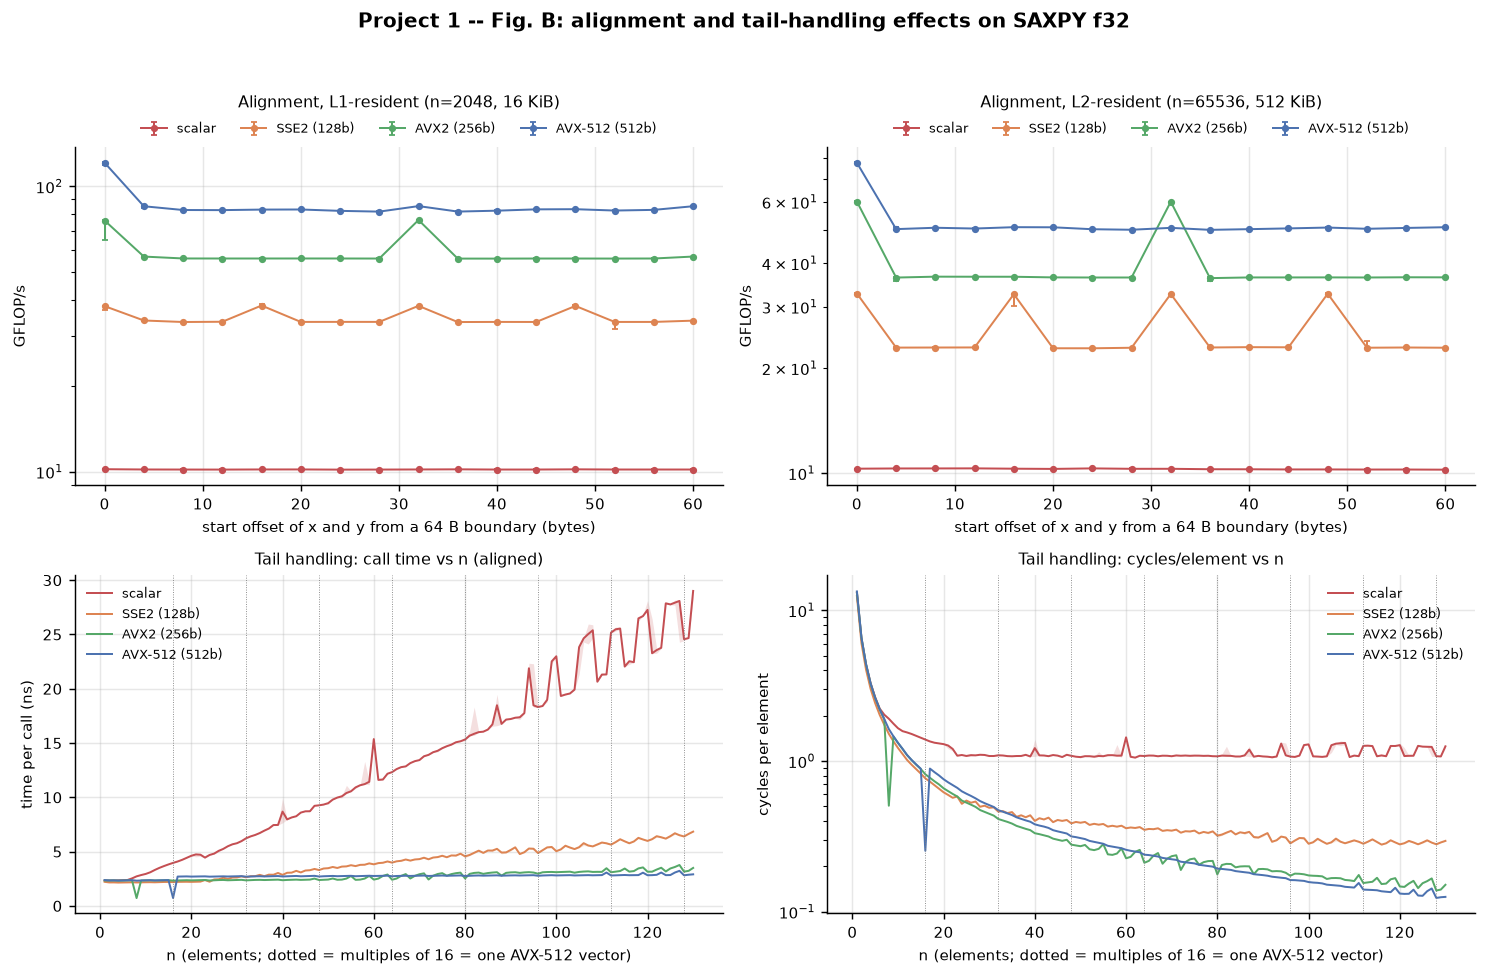
\includegraphics[width=0.94\linewidth]{../results/figB_alignment_and_tail.png}
\caption{Top: SAXPY throughput against the byte offset of $x$ and $y$ from a 64\,B boundary, L1- and L2-resident. Bottom: call time and cycles per element for $n=1$ to 130, aligned; dotted lines mark multiples of 16.}\label{fig:B}\end{figure}
\textbf{Alignment.} A misaligned start makes some loads and stores straddle two cache lines: one in four for SSE2, one in two for AVX2 and every access for AVX-512. The penalty grows in that order (Tab.~\ref{tab:tail}, Fig.~\ref{fig:B} top), less than proportionally for AVX-512, possibly because its aligned loop is already limited by L1 bandwidth.
\begin{table}[H]\centering\small\begin{tabular}{lrrrrrr}
\toprule
build & $t(16)$ ns & $t(15)$ ns & $t(17)$ ns & $t(128)$ ns & $t(127)$ ns & misaligned penalty (L1) \\
\midrule
scalar & 3.96 & 3.82 & 4.09 & 24.57 & 28.09 & 0\% \\
SSE2 (128b) & 2.19 & 2.21 & 2.21 & 6.40 & 6.51 & 12\% \\
AVX2 (256b) & 2.33 & 2.37 & 2.34 & 3.16 & 3.77 & 26\% \\
AVX-512 (512b) & 0.72 & 2.38 & 2.70 & 2.82 & 3.23 & 32\% \\
\bottomrule
\end{tabular}

\caption{Call time $t(n)$ in ns for aligned arrays around one vector length, and the median penalty of the 15 misaligned offsets in L1.}\label{tab:tail}\end{table}
\textbf{Tail.} In the first experiment an AVX-512 call with $n=16$ is fast and every other size, even $n=32$ and 48, which have no tail, is about 2\,ns slower (Tab.~\ref{tab:tail}, Fig.~\ref{fig:B} bottom). The first thing verified was if this was because of the masked tail, which was incorrect. The benchmark calls the kernel repeatedly on the same \texttt{y}, so each call waits for the previous call's stores. Rotating through 64 output buffers (\texttt{exp3b}) removes that dependency; every size then takes about 7 cycles and the tail adds only 0.2--4 cycles (Tab.~\ref{tab:tailrot}). The fast $n=16$ point repeats in all three runs but not in an exact replica of the harness, so it depends on how the compiler built that call; This was not investigated further. For long arrays the tail is invisible.
\begin{table}[H]\centering\small\resizebox{0.85\linewidth}{!}{\begin{tabular}{rrrrrr}
\toprule
$n$ & remainder (lanes) & same $y$ every call (ns) & 64 rotating $y$ buffers (ns) & cycles, rotating & rotating, minus the multiple of 16 below \\
\midrule
8 & 8 & 2.32 & 1.27 & 7.1 & -- \\
15 & 15 & 2.37 & 1.48 & 8.3 & +0.21 ns \\
16 & 0 & 2.68 & 1.26 & 7.1 & -- \\
17 & 1 & 2.70 & 1.29 & 7.2 & +0.03 ns \\
31 & 15 & 2.73 & 1.74 & 9.7 & +0.47 ns \\
32 & 0 & 2.70 & 1.28 & 7.2 & -- \\
33 & 1 & 2.71 & 1.32 & 7.4 & +0.04 ns \\
47 & 15 & 2.77 & 1.98 & 11.1 & +0.70 ns \\
48 & 0 & 2.72 & 1.30 & 7.3 & -- \\
49 & 1 & 2.74 & 1.51 & 8.4 & +0.20 ns \\
\bottomrule
\end{tabular}
}
\caption{AVX-512 SAXPY call time for short vectors, median of 21 batches: the same $y$ on every call against 64 rotating $y$ buffers that stay in L1. The last column is the cost of the masked tail, the rotating time minus that of the multiple of 16 below.}\label{tab:tailrot}\end{table}

\subsection{Stride and gather}\label{sec:stride}
\begin{figure}[!htb]\centering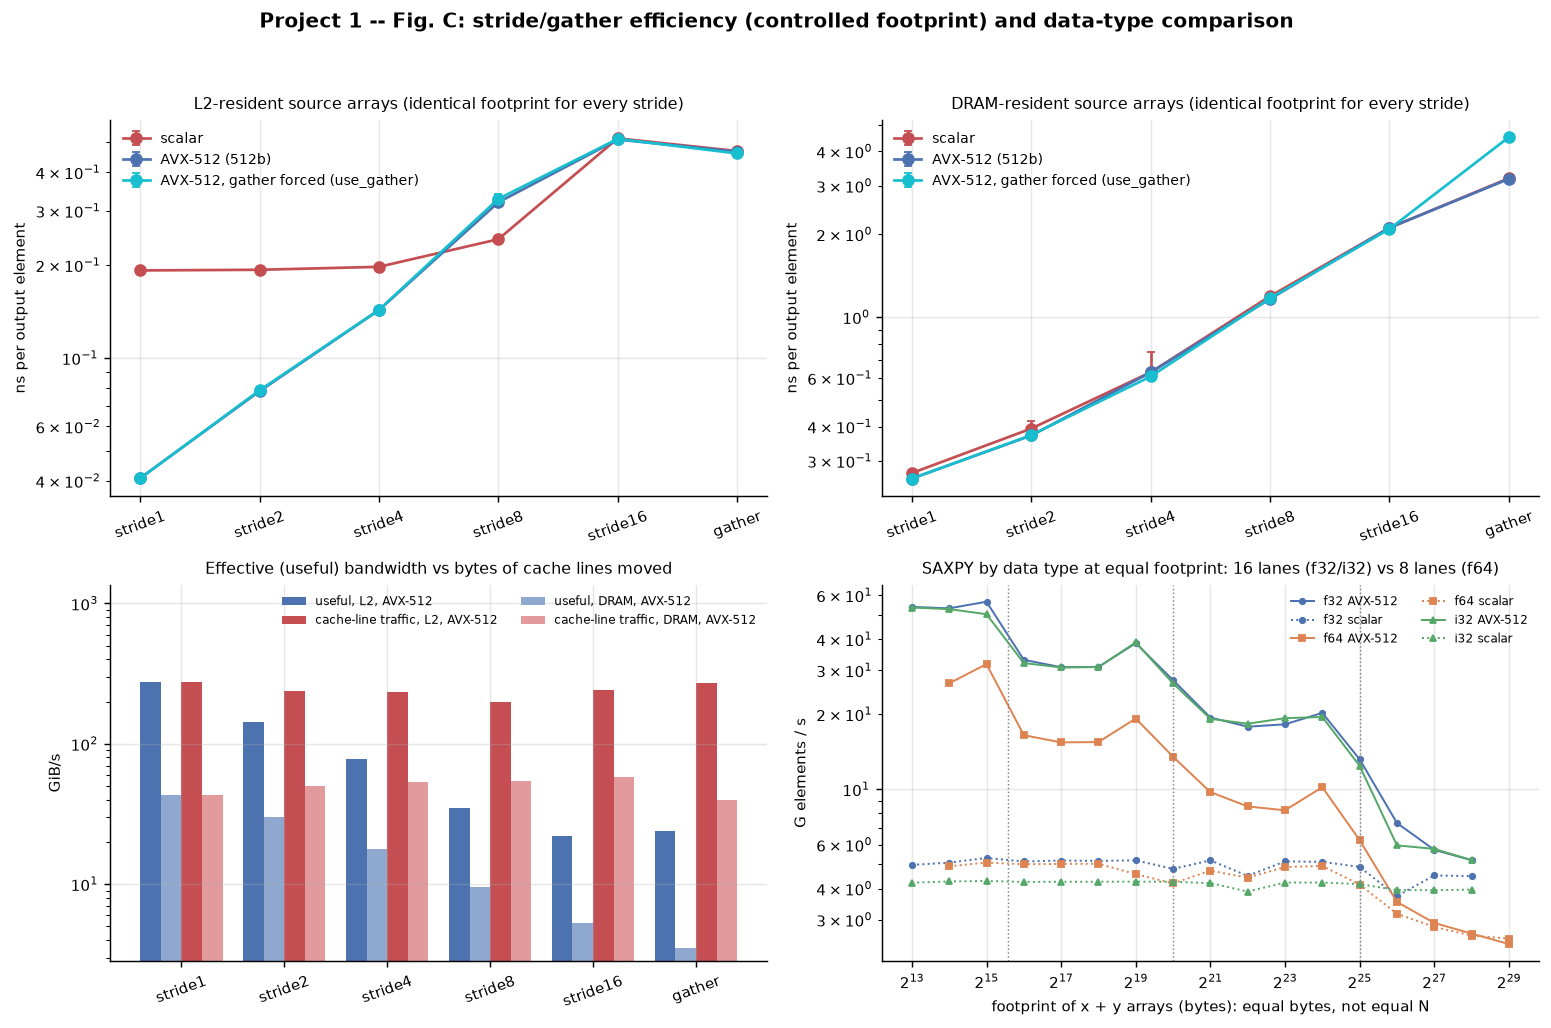
\includegraphics[width=\linewidth]{../results/figC_stride_gather_and_dtype.png}
\caption{Top: time per output element of $z_i=x_{iS}\,y_{iS}$ for strides $S=1$ to 16 and a random gather at a fixed array footprint, L2- and DRAM-resident. Bottom left: useful bandwidth against the bytes of cache lines touched. Bottom right: SAXPY by data type at equal footprint.}\label{fig:C}\end{figure}
The footprint stays fixed as the stride grows, so each fetched 64-byte line yields fewer useful elements (Fig.~\ref{fig:C}). With L2-resident data the AVX-512 advantage falls from almost 5$\times$ at stride 1 to 1.4$\times$ at stride 4; AVX-512 is slower than scalar at stride 8, and the two tie at stride 16 and for the gather, which gcc leaves scalar. With DRAM-resident data scalar and SIMD tie at every stride: line traffic stays near the DRAM limit while useful bandwidth falls, so at stride 16 about 90\% of the delivered bytes go unused. Forcing the \texttt{vgatherdps} gather changes nothing in L2 and is 42\% slower in DRAM, which supports gcc's choice not to emit gathers here. The stride-8 and gather results reflect gcc's cost model and Zen~5's gather hardware, not SIMD code in general.

\subsection{Data type}\label{sec:dtype}
\begin{table}[!htb]\centering\small\begin{tabular}{llrrrrr}
\toprule
kernel & dtype (lanes) & \multicolumn{2}{c}{L1 (32 KiB of x+y)} & \multicolumn{2}{c}{DRAM (256 MiB of x+y)} & \\
 & & AVX-512 Gelem/s & speedup & AVX-512 Gelem/s & speedup & \\
\midrule
saxpy & f32 (16) & 56.58 & 10.7$\times$ & 5.20 & 1.2$\times$ & \\
 & f64 (8) & 31.81 & 6.3$\times$ & 2.64 & 1.0$\times$ & \\
 & i32 (16) & 50.42 & 11.8$\times$ & 5.20 & 1.3$\times$ & \\
\addlinespace
mul & f32 (16) & 54.50 & 10.7$\times$ & 3.81 & 1.1$\times$ & \\
 & f64 (8) & 24.56 & 4.7$\times$ & 1.92 & 1.0$\times$ & \\
 & i32 (16) & 54.50 & 12.8$\times$ & 3.82 & 1.1$\times$ & \\
\addlinespace
dot & f32 (16) & 2.68 & 1.0$\times$ & 2.66 & 1.0$\times$ & \\
 & f64 (8) & 2.75 & 1.0$\times$ & 2.59 & 1.0$\times$ & \\
 & i32 (16) & 56.04 & 13.3$\times$ & 7.20 & 1.8$\times$ & \\
\addlinespace
\bottomrule
\end{tabular}

\caption{AVX-512 throughput in billions of elements per second and speedup over scalar at equal footprint, so f64 uses half as many elements. i32 is a 32-bit unsigned integer.}\label{tab:dtype}\end{table}
At equal bytes in L1, f32 and i32 have 16 lanes and similar element rates, while f64, with 8 lanes, reaches a little over half that (Tab.~\ref{tab:dtype}, Fig.~\ref{fig:C} bottom right). In DRAM all types hit the same byte rate, so f64 delivers half as many elements per second: bytes per element, not lane count, decide there. Both limits predict the same halving: a 512-bit FMA costs the same for f32 and f64 but covers half as many f64 elements, and 8-byte elements halve the arithmetic intensity, from 0.167 to 0.083 FLOP/B for SAXPY, so the DRAM roof also delivers half the FLOP. Operation cost matters little here. The integer SAXPY, which uses a run-time multiplier so gcc cannot replace the multiply with shifts, needs a separate multiply and add because AVX-512 has no 32-bit integer FMA, yet it reaches about 90\% of the f32 rate in L1: loads and stores, not arithmetic, limit both types. The integer dot product gains from SIMD because integer addition is associative; the floating-point dot products do not (Sec.~\ref{sec:neg}).

\subsection{Roofline}\label{sec:roofline}
\begin{figure}[!htb]\centering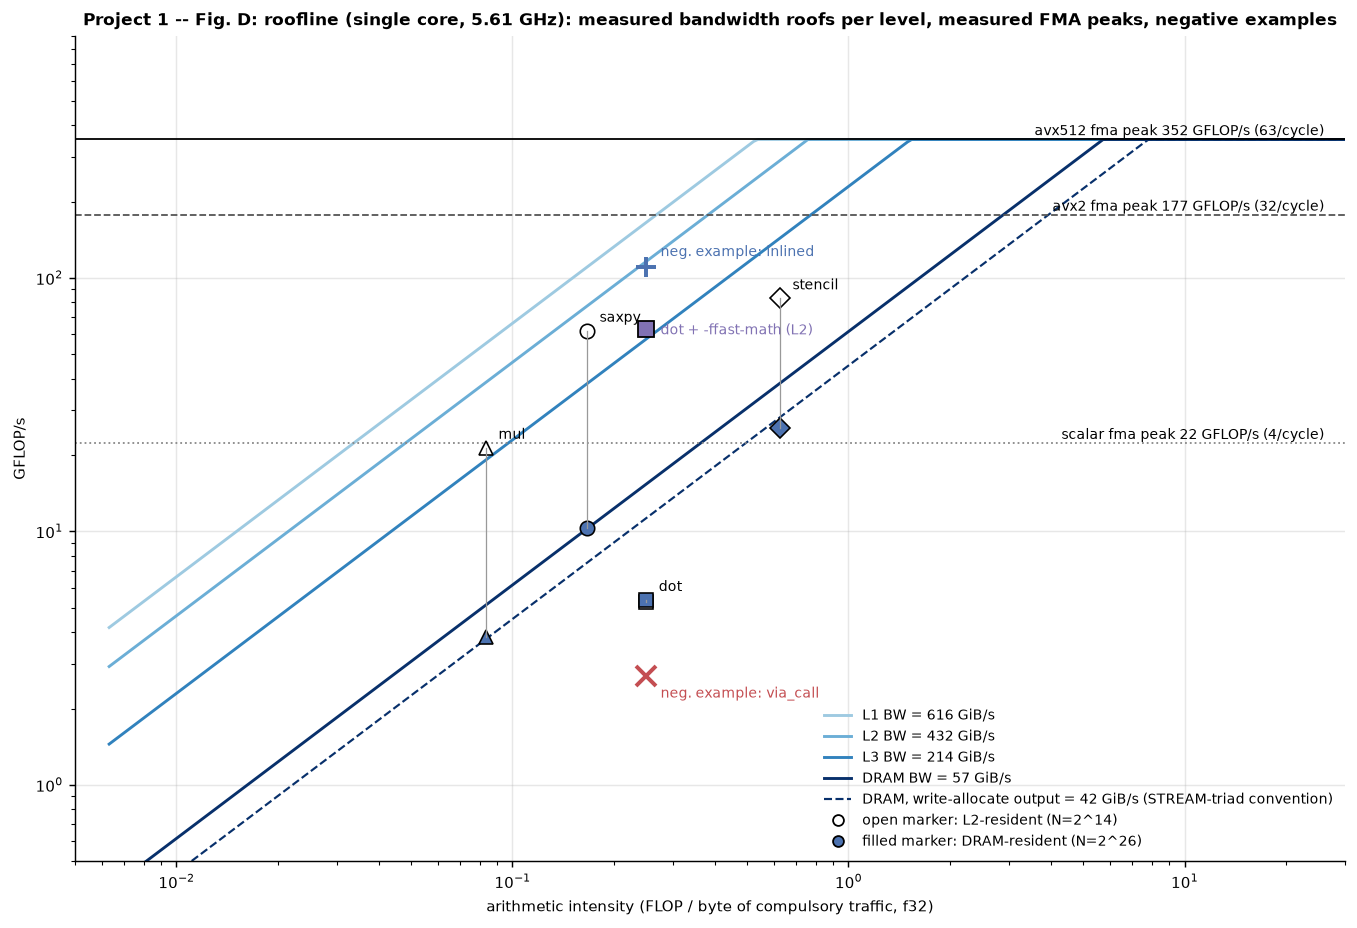
\includegraphics[width=0.85\linewidth]{../results/figD_roofline_and_negative_example.png}
\caption{Single-core roofline, f32. Solid roofs are the measured streaming bandwidth of each level, the dashed roof is DRAM with a separate output array, and horizontal roofs are the measured FMA peaks. Open markers are L2-resident, filled markers DRAM-resident.}\label{fig:D}\end{figure}
\begin{table}[!htb]\centering\small\begin{tabular}{lrrr}
\toprule
level & triad GiB/s (12 B/elem) & read-only GiB/s & footprint band \\
\midrule
L1 & 616.1 & 302.5 & 6--40 KiB \\
L2 & 432.3 & 169.2 & 100--700 KiB \\
L3 & 213.6 & 149.6 & 2--8 MiB \\
DRAM & 57.2 & 53.2 & $\geq$ 300 MB \\
\midrule
ISA & measured GFLOP/s & FLOP/cycle & lanes (f32) \\
\midrule
scalar\_fma & 22.3 & 4.0 & 1 \\
sse\_fma & 88.9 & 15.9 & 4 \\
avx2\_fma & 177.0 & 31.6 & 8 \\
avx512\_fma & 351.7 & 62.9 & 16 \\
\bottomrule
\end{tabular}

\caption{Measured ceilings. Bandwidth roofs are the best of three streaming kernels in each footprint band; FMA peaks come from register-resident code with 16 independent accumulators.}\label{tab:ceil}\end{table}
\begin{table}[!htb]\centering\scriptsize\begin{tabular}{llllrrrrrr}
\toprule
kernel & level & build & roof says & intensity & achieved & roof & \% of roof & true traffic & \% of level bandwidth \\
 & & & & FLOP/B & GFLOP/s & GFLOP/s & & GiB/s & \\
\midrule
saxpy & L2 & scalar & compute & 0.167 & 10.3 & 22.3 & 46\% & 57.6 & 13\% \\
saxpy & L2 & avx512 & memory & 0.167 & 61.8 & 77.4 & 80\% & 345.5 & 80\% \\
saxpy & DRAM & scalar & memory & 0.167 & 8.8 & 10.2 & 86\% & 49.2 & 86\% \\
saxpy & DRAM & avx512 & memory & 0.167 & 10.3 & 10.2 & 101\% & 57.5 & 101\% \\
\addlinespace
dot & L2 & scalar & compute & 0.250 & 5.5 & 22.3 & 25\% & 20.6 & 5\% \\
dot & L2 & avx512 & memory & 0.250 & 5.3 & 116.0 & 5\% & 19.6 & 5\% \\
dot & L2 & avx512\_fm & memory & 0.250 & 62.9 & 116.0 & 54\% & 234.4 & 54\% \\
dot & DRAM & scalar & memory & 0.250 & 5.5 & 15.3 & 36\% & 20.3 & 36\% \\
dot & DRAM & avx512 & memory & 0.250 & 5.4 & 15.3 & 35\% & 20.0 & 35\% \\
dot & DRAM & avx512\_fm & memory & 0.250 & 14.1 & 15.3 & 92\% & 52.5 & 92\% \\
\addlinespace
mul & L2 & scalar & compute & 0.083 & 5.1 & 22.3 & 23\% & 76.7 & 18\% \\
mul & L2 & avx512 & memory & 0.083 & 21.4 & 38.7 & 55\% & 318.2 & 74\% \\
mul & DRAM & scalar & memory & 0.083 & 3.7 & 5.1 & 71\% & 54.4 & 95\% \\
mul & DRAM & avx512 & memory & 0.083 & 3.8 & 5.1 & 75\% & 57.2 & 100\% \\
\addlinespace
stencil & L2 & scalar & compute & 0.625 & 21.6 & 22.3 & 97\% & 48.3 & 11\% \\
stencil & L2 & avx512 & memory & 0.625 & 83.0 & 290.1 & 29\% & 185.5 & 43\% \\
stencil & DRAM & scalar & compute & 0.625 & 20.1 & 22.3 & 90\% & 44.8 & 78\% \\
stencil & DRAM & avx512 & memory & 0.625 & 25.7 & 38.4 & 67\% & 57.4 & 100\% \\
\bottomrule
\end{tabular}

\caption{Where each kernel sits, f32. True traffic includes write-allocate reads; the last column is relative to the measured streaming bandwidth of the footprint's level.}\label{tab:roofline}\end{table}
The roofline model \cite{roofline} bounds the attainable rate by $\min(\text{peak FLOP/s},\ \text{arithmetic intensity}\times\text{bandwidth})$, with intensity in FLOP per byte of traffic; every roof is measured on this machine (Tab.~\ref{tab:ceil}, Fig.~\ref{fig:D}). At DRAM size the AVX-512 SAXPY, multiply and stencil run at the measured DRAM bandwidth once write-allocate traffic is counted, so they are memory-bound (Tab.~\ref{tab:roofline}). For SAXPY the model bounds the SIMD speedup at $57/49 = 1.16\times$, matching the measured $1.17\times$. In L1 and L2 no AVX-512 kernel reaches the compute roof: low arithmetic intensity keeps them on the bandwidth slopes. The dot product is far from both roofs because it is latency-bound; with \texttt{-ffast-math} it approaches the DRAM roof. All roofs are single-core; Project~2 shows that several cores draw more DRAM bandwidth.

\subsection{Hardware counters}\label{sec:counters}
\begin{table}[!htb]\centering\small\resizebox{0.8\linewidth}{!}{\begin{tabular}{llrrrrr}
\toprule
kernel (f32, L1) & build & instr./elem & reduction vs.\ scalar & cycles/elem & IPC & loads/elem \\
\midrule
saxpy & scalar & 6.008 & 1.0$\times$ & 1.050 & 5.72 & 3.002 \\
 & sse2 & 2.009 & 3.0$\times$ & 0.271 & 7.42 & 0.757 \\
 & avx2 & 0.759 & 7.9$\times$ & 0.139 & 5.45 & 0.381 \\
 & avx512 & 0.385 & 15.6$\times$ & 0.100 & 3.87 & 0.189 \\
\addlinespace
mul & scalar & 6.024 & 1.0$\times$ & 1.028 & 5.86 & 3.008 \\
 & sse2 & 1.781 & 3.4$\times$ & 0.269 & 6.62 & 0.761 \\
 & avx2 & 0.781 & 7.7$\times$ & 0.146 & 5.35 & 0.384 \\
 & avx512 & 0.409 & 14.7$\times$ & 0.089 & 4.58 & 0.200 \\
\addlinespace
stencil & scalar & 7.004 & 1.0$\times$ & 1.500 & 4.67 & 2.004 \\
 & sse2 & 3.021 & 2.3$\times$ & 0.597 & 5.06 & 1.196 \\
 & avx2 & 0.904 & 7.7$\times$ & 0.456 & 1.98 & 0.700 \\
 & avx512 & 0.454 & 15.4$\times$ & 0.380 & 1.19 & 0.445 \\
\addlinespace
dot & scalar & 6.011 & 1.0$\times$ & 1.944 & 3.09 & 2.004 \\
 & sse2 & 3.765 & 1.6$\times$ & 1.946 & 1.93 & 0.504 \\
 & avx2 & 2.513 & 2.4$\times$ & 1.943 & 1.29 & 0.254 \\
 & avx512 & 2.263 & 2.7$\times$ & 1.999 & 1.13 & 0.128 \\
 & avx512-fm & 0.207 & 29.0$\times$ & 0.064 & 3.24 & 0.128 \\
\addlinespace
\bottomrule
\end{tabular}
}
\caption{Retired instructions, cycles and loads per element, f32, L1-resident ($n=2048$, three arrays totalling 24\,KiB). One run per row; the reduction is the scalar instruction count divided by that of the build.}\label{tab:cinstr}\end{table}
\begin{table}[!htb]\centering\small\resizebox{\linewidth}{!}{\begin{tabular}{lrrrrr}
\toprule
kernel (f32, 384 MiB) & model: line reads (B/elem) & measured scalar & measured AVX-512 & DRAM share of fills & cycles/elem scalar $\rightarrow$ AVX-512 \\
\midrule
saxpy & 8 & 8.02 & 8.06 & 71\% & 1.22 $\rightarrow$ 1.06 \\
mul & 12 & 12.04 & 12.14 & 90\% & 1.43 $\rightarrow$ 1.46 \\
stencil & 8 & 8.02 & 8.03 & 60\% & 1.55 $\rightarrow$ 1.05 \\
dot & 8 & 8.02 & 8.02 & 0\% & 2.02 $\rightarrow$ 2.07 \\
\bottomrule
\end{tabular}
}
\caption{Cache-line fills per element at DRAM size, three arrays of 128\,MiB, summed over L2, L3 and DRAM as sources. The DRAM share differs between kernels only because the hardware prefetcher stages lines in L2 first when the loop is slow enough.}\label{tab:ctraffic}\end{table}
Hardware counters prove SIMD actually happened. Retired instructions per element fall by close to the lane count for AVX2 and AVX-512 (Tab.~\ref{tab:cinstr}). SSE2 falls short because the \texttt{-march=x86-64} target has no FMA, so each iteration needs a separate multiply and add. The scalar loop's instructions per cycle (IPC) stay below Zen~5's 8-wide retire \cite{amdhc}, so scalar code is limited by its own instruction stream, not by memory, which is why the L1 gain is large. The ``vectorized'' float dot retires fewer instructions but needs the same 2 cycles per element in every build; with \texttt{-ffast-math} both drop by about 30$\times$ (Sec.~\ref{sec:neg}).

At DRAM size the line fills match the roofline model's read traffic within about 1\% and are the same for scalar and AVX-512 (Tab.~\ref{tab:ctraffic}): SIMD changes the instruction count but not the traffic, which is the roofline's memory-bound argument. The counters cannot see write-backs, so full DRAM bandwidth for multiply and the stencil still assumes each output line is written back once.

\section{Negative cases and anomalies}\label{sec:negan}
\subsection{Negative and misleading cases}\label{sec:neg}
\textbf{(1) Floating-point dot product: reported as vectorized, but not faster than scalar.} The dot kernel adds every product $x_i y_i$ into one running sum. gcc reports the loop as vectorized with 64-byte vectors, yet all four builds run at about 2 cycles per element at every size. Because C++ fixes the order of floating-point additions, the 16 products of each vector are added to the sum one at a time (Sec.~\ref{sec:verify}); each add waits for the previous one, and an add takes 2 cycles on Zen~5. The counters agree: fewer instructions, same cycles (Sec.~\ref{sec:counters}). \emph{Test:} \texttt{-ffast-math} \cite{gccdoc} allows reordering, so gcc keeps independent partial sums in separate vector registers. The speedup becomes about 29$\times$ in L1, shrinking to 2.6$\times$ in DRAM (Tab.~\ref{tab:speedup}), at the cost of different rounding within the validation tolerance. The integer dot product vectorizes without the flag, because integer addition gives the same result in any order.

\textbf{(2) Looks easy to vectorize, but is not: a loop that calls a function gcc cannot see into.} Two loops compute the same $y_i = 1.0000001\,x_i + 10^{-7}$. The first gets each element from a function compiled in a separate file, \texttt{black\_box.cpp}, with link-time optimization off; gcc cannot see what it does, leaves the loop scalar and reports that the call ``can throw an exception''. The second writes the arithmetic in the loop body and is vectorized. It is 39$\times$ faster in L1 but only about 4$\times$ in DRAM, so a missed vectorization is easy to overlook when only memory-bound sizes are measured.

\textbf{(3) Vectorized, but little gain: memory-bound loops.} SAXPY, multiply and the stencil vectorize at every size, but with DRAM-resident arrays the scalar loops already use most of the bandwidth (Sec.~\ref{sec:roofline}). Memory also sets the speed where AVX-512 is slower than scalar at stride 8 in L2 and where forced gathers lose in DRAM (Sec.~\ref{sec:stride}), and where AVX-512 is no faster than AVX2 at 60--300\,KiB (Sec.~\ref{sec:locality}).

\subsection{Honest anomalies}\label{sec:anomalies}
\begin{itemize}
  \item \textbf{Clock.} For some runs the CPU experienced clock speeds lower than the 5.61\,GHz the pinned core usually sustains. The 27 clock samples of the three runs span 5.56--5.62\,GHz, at most 1\% below the 5.61\,GHz used for every cycles-per-element value, so those values are off by at most about 1\%. This variation is probably due to Windows 11 processes spinning up on other cores. AMD's boost algorithm raises the clock speed according to limits, one of which is current draw \cite{amdpb2}. If other cores are drawing current away from the benchmarked core, that would cause variation in clock speed, in my experience, thermal throttling usually results in greater variation, and temperature did not get above 95 degrees C while trying to isolate the cause of this, the most likely scenario attributes it to current draw.
  \item \textbf{A stencil spike at one L1 size and a SAXPY bump at 300--700\,KiB}, both AVX-512 only, proved difficult to isolate with Windows counters. L2 prefetcher or cache-set conflicts at particular array offsets are possible causes.
  \item \textbf{Multiply gains less than the lane count even in L1}, possibly because it already runs at the measured L1 bandwidth roof.
\end{itemize}

\section{Use of artificial intelligence (AI)}\label{sec:aiuse}


Since Professor Tong Zhang has been encouraging the use of AI for learning, with an emphasis on how to best leverage it, I made an effort to experiment with the boundaries of how I used AI in this assignment.

 Throughout this process, I used AI to teach myself about deeper technical detail concerning report topics. I used a mix of Qwen 3.8 running locally via OpenCode to build the repository and code. I used Claude Opus 5.0, 5.1, and 5.5 (they came out over the course of this semester) for technical questions.

 Once I had a pipeline for getting results, I was able to independently tweak benchmarks and draw conclusions about my hypotheses. I rejected some charts that didn't make sense to me, and got the AI to combine other charts so data could be better viewed side by side.

 I experimented with AI use beyond writing the benchmark code to varying degrees of success. One thing that went well was using Qwen to make charts and tables, most scripts that do this were written by Qwen.

 One AI experiment that went wrong was when it came time to compile the final report from my independent hypotheses and findings. I gave Claude the documents and charts, and it immediately made 100+ pages of report across 3 projects. After a signifigant number of AI and human independent revisions, I managed to get this down to a more digestible $\approx$~40 pages accross all 3 projects. \textbf{This includes the clickable guides in the appendix, which were generated by AI to make the report more legible from the perspective of the handout, for easy grading.}


\begin{thebibliography}{9}
\raggedright\small
\bibitem{course} ECSE 4320/6320 Advanced Computer Systems, \emph{Class-wide Projects} (course document, due October 16): requirements and grading rubrics.
\bibitem{roofline} S.~Williams, A.~Waterman, D.~Patterson, ``Roofline: an insightful visual performance model for multicore architectures,'' \emph{Communications of the ACM} 52(4), 65--76, 2009. doi:10.1145/1498765.1498785.
\bibitem{amdhc} Cohen and Subramony (AMD), ``Next generation `Zen~5' core,'' Hot Chips 2024, \url{https://www.hc2024.hotchips.org/assets/program/conference/day2/24_HC2024.AMD.Cohen.Subramony.final.pdf}, slides 4 and 8--10: cache sizes, 8-wide retire, two 512-bit FMA pipes, 2-cycle FADD.
\bibitem{amdpb2} AMD, ``AMD Ryzen Technology: Precision Boost 2 Performance Enhancement,'' support article CPU-PB2, \url{https://www.amd.com/en/resources/support-articles/faqs/cpu-pb2.html}: boost is limited by temperature, active cores, socket power and current draw.
\bibitem{chips9950x} Chips and Cheese, ``AMD's Ryzen 9950X: Zen 5 on desktop'' (2024), \url{https://chipsandcheese.com/p/amds-ryzen-9950x-zen-5-on-desktop}: 32\,MB of L3 per CCD.
\bibitem{perfzen5} Linux kernel, AMD Zen~5 event definitions (\texttt{ls\_any\_fills\_from\_sys}, \texttt{ls\_l1\_d\_tlb\_miss}), \url{https://github.com/torvalds/linux/blob/master/tools/perf/pmu-events/arch/x86/amdzen5/load-store.json}.
\bibitem{gccdoc} GCC manual, \emph{Options That Control Optimization}, \url{https://gcc.gnu.org/onlinedocs/gcc/Optimize-Options.html}: \texttt{-ffast-math} enables \texttt{-fassociative-math} through \texttt{-funsafe-math-optimizations}; \texttt{-fopt-info} is under \emph{Developer Options}, \url{https://gcc.gnu.org/onlinedocs/gcc/Developer-Options.html}.
\end{thebibliography}

\appendix
\section{Summary of results}\label{sec:summary}
{\small
\begin{tabular}{p{4.0cm}p{12.1cm}}
\toprule
\textbf{Question} & \textbf{Answer (evidence)} \\
\midrule
How large is the gain? & In L1, AVX-512 code is about ten times faster than scalar code for SAXPY and multiply, and about eight times for the stencil; narrower builds gain less (Tab.~\ref{tab:speedup}, Fig.~\ref{fig:A}). \\
Where does it compress? & At every cache boundary. In DRAM the scalar loop already uses most of the bandwidth, so little gain is left (Tab.~\ref{tab:roofline}). \\
Is wider always better? & No. AVX2 and AVX-512 run at the same speed while the data sit in L2, because L2 bandwidth is the limit (Sec.~\ref{sec:locality}). \\
Misalignment and tail? & Misalignment costs more as vectors widen, about a third for AVX-512. The masked tail costs only a few cycles; a larger jump first blamed on it comes from a dependency between consecutive calls (Tab.~\ref{tab:tailrot}, Fig.~\ref{fig:B}). \\
Stride and gather? & SIMD helps only at small strides, is slower than scalar at stride 8 in L2 and gains nothing on gathers. Forced hardware gathers are slower in DRAM (Fig.~\ref{fig:C}). \\
Data type? & In L1, f64 reaches about half the element rate of f32, matching its half lane count; in DRAM all types hit the same byte rate. Integer dot gains from SIMD, floating-point dot does not (Tab.~\ref{tab:dtype}). \\
Negative cases & A floating-point dot reported as vectorized with no gain, a loop that calls a function the compiler cannot see into and is not vectorized, and DRAM-bound loops that vectorize with little gain (Sec.~\ref{sec:neg}). \\
Counters & Instructions per element fall by nearly the lane count for AVX2 and AVX-512 and by less for SSE2. The floating-point dot retires fewer instructions in the same number of cycles. Cache-line fills match the traffic model and are the same for scalar and SIMD (Tab.~\ref{tab:cinstr}, \ref{tab:ctraffic}). \\
\bottomrule
\end{tabular}
}

\section{Where the rubric categories are answered}\label{sec:rubric}
\begin{center}\small
\begin{tabular}{p{6.0cm}rp{7.6cm}}
\toprule
\textbf{Rubric category} & \textbf{Points} & \textbf{Location} \\
\midrule
Baseline, correctness, reproducibility & 15 & Sec.~\ref{sec:repro} (commands, run-to-run variation), \ref{sec:platform} (baseline setup), \ref{sec:valid} (validation) \\
Vectorization verification & 15 & Sec.~\ref{sec:verify} (reports, disassembly), \ref{sec:counters} (counters) \\
Locality and memory-bound analysis & 20 & Sec.~\ref{sec:locality}, \ref{sec:roofline} \\
Alignment, tail, stride/gather studies & 20 & Sec.~\ref{sec:align}, \ref{sec:stride} \\
Roofline and quantitative insight & 20 & Sec.~\ref{sec:roofline}, \ref{sec:dtype}, \ref{sec:counters} \\
AI use transparency and failure case & 10 & Sec.~\ref{sec:aiuse} (AI use), \ref{sec:neg} (failure cases) \\
Report quality & 10 & whole report; checklist in App.~\ref{sec:checklist} \\
\bottomrule
\end{tabular}
\end{center}

\section{Requirements checklist}\label{sec:checklist}
Every requirement of the course document \cite{course} for Project~1 and its common requirements, with the section that answers it. \textbf{Met} = done and documented; \textbf{Not met} = not done and the reason is stated.
\begin{center}\footnotesize
\begin{longtable}{p{6.3cm}p{1.5cm}p{7.7cm}}
\toprule
\textbf{Requirement} & \textbf{Status} & \textbf{Where / evidence} \\
\midrule
\endhead
\multicolumn{3}{l}{\textit{Common requirements}} \\
AI-use note (tools, what was generated, what was modified/tested/rejected) & Met & Sec.~\ref{sec:aiuse} \\
Reproducible repository: source, build scripts, run scripts, plotting scripts, raw data, processed data, README & Met & \texttt{src/}, \texttt{scripts/}, \texttt{data/raw|repeats|processed}, \texttt{README.md}; commands in Sec.~\ref{sec:repro} \\
Pre-experiment hypothesis (expected trend and why) & Met & Sec.~\ref{sec:hyp}: six hypotheses and their outcome \\
Correctness validation against a simple reference or sanity checks & Met & Sec.~\ref{sec:valid} (reference loops, long-double accumulation, canaries) \\
Measurement discipline: hardware, OS, compiler/tool versions, frequency, SMT, pinning, repetitions, error bars & Met & Sec.~\ref{sec:platform} (platform table; interquartile-range bands in every figure; 3 independent runs) \\
Negative/failure case & Met & Sec.~\ref{sec:neg} (three, each verified) \\
Honest anomalies with hypotheses & Met & Sec.~\ref{sec:anomalies} \\
Optional graphics processing unit (GPU)/CUDA extension & Not attempted & optional; no CUDA toolkit/MSVC on this machine \\
\midrule
\multicolumn{3}{l}{\textit{Scope and tools}} \\
Required experiments single-threaded & Met & all experiments pinned to one logical CPU \\
GCC/Clang with optimization; exact compiler versions and flags recorded & Met & g++ 16.2.0, flag table in Sec.~\ref{sec:verify}, \texttt{results/build\_flags.txt} \\
Compiler vectorization reports and/or disassembly & Met & Sec.~\ref{sec:verify} \\
Reliable timing and statistics; runtime, GFLOP/s or GiB/s, cycles per element & Met & all figures/tables; cycles/element with the measured clock \\
Recommended: perf or similar counters (instructions, vector instructions, cache misses, memory traffic) & Met & Sec.~\ref{sec:countermethod}, \ref{sec:counters}: retired instructions, cycles, loads, L1D fills by source (memory traffic); no vector-instruction counter, so vector use is shown by instruction-count ratios and disassembly \\
\midrule
\multicolumn{3}{l}{\textit{Kernel set (at least three) and knobs}} \\
Kernels: SAXPY, dot, elementwise multiply, 3-point stencil & Met & all four, Sec.~\ref{sec:locality} \\
Data type f32 vs.\ f64 (optionally i32) & Met & f32, f64 and i32; Tab.~\ref{tab:dtype} \\
Alignment (shifted start) and tail (sizes with/without vector-width remainders) & Met & 16 offsets $\times$ L1/L2; $n=1..130$; Sec.~\ref{sec:align} \\
Access pattern: unit stride, stride 2/4/8/16, gather-like & Met & Sec.~\ref{sec:stride} \\
Working-set sweep across L1, L2, LLC, DRAM & Met & $N=2^{10}..2^{26}$, Sec.~\ref{sec:locality} \\
Compiler/ISA flags: scalar-only, default auto-vectorized, CPU-targeted widest & Met & scalar / SSE2 (default) / AVX2 / AVX-512 / +fast-math / +forced gather \\
\midrule
\multicolumn{3}{l}{\textit{Required experiments and plots}} \\
Scalar baseline vs.\ auto-vectorized for each kernel across sizes (speedup, throughput) & Met & Fig.~\ref{fig:A}, Tab.~\ref{tab:speedup} \\
Locality sweep for one kernel, annotated where SIMD gains compress & Met & Sec.~\ref{sec:locality}, Fig.~\ref{fig:A} (bottom) \\
Alignment and tail-handling study (prologue/epilogue, unaligned, masking) & Met & Fig.~\ref{fig:B}, Tab.~\ref{tab:tail}, \ref{tab:tailrot} \\
Stride/gather study (effective bandwidth, SIMD efficiency) & Met & Fig.~\ref{fig:C} \\
Data-type comparison (lanes, arithmetic intensity, operation cost) & Met & Tab.~\ref{tab:dtype}, Sec.~\ref{sec:dtype} (lanes, intensity, integer multiply-add vs.\ FMA) \\
Vectorization verification (concise report/disassembly, no full dumps) & Met & Sec.~\ref{sec:verify} \\
Roofline for $\ge$1 kernel with measured memory bandwidth and estimated CPU peak FLOP rate & Met & Fig.~\ref{fig:D}, Tab.~\ref{tab:ceil}, \ref{tab:roofline} (all four kernels; measured, not estimated, FMA peaks) \\
One negative example, verified and explained & Met & Sec.~\ref{sec:neg} \\
\midrule
\multicolumn{3}{l}{\textit{Deliverables}} \\
Methodology: CPU model/ISA, compiler and flags, OS, frequency policy, SMT, timing, repetitions, data initialization & Met & Sec.~\ref{sec:method} \\
Plots/tables with units, legends, variability & Met & all figures \\
Short report linking results to locality, vector width, arithmetic intensity, bandwidth, anomalies & Met & this report \\
\bottomrule
\end{longtable}
\end{center}

\end{document}
